\documentclass[12pt]{report}
\usepackage[utf8]{inputenc}
\usepackage{graphicx}
\usepackage{float}
\usepackage{listings}
\usepackage{titlesec}
\usepackage{xcolor}
\usepackage{fancyhdr}
\usepackage[pdfborder={0 0 0}]{hyperref} 
\usepackage{silence}
\usepackage{tikz}
\usepackage{charter}
\usepackage[table]{xcolor} 
\usepackage{float}  
\usepackage{longtable}          
\usepackage{atbegshi} 
\usepackage{array}
\usepackage{cellspace}
\usepackage[a4paper, left=1in, right=1in, bottom=0.8in, top=0.8in]{geometry}
\usepackage{tikz}
\usepackage{pgf-umlsd}
\newlength{\mymargin}
\setlength{\mymargin}{0.8cm}
\renewcommand{\baselinestretch}{1.4}
\pagenumbering{gobble}  % disable page numbering
\setlength{\cellspacetoplimit}{6pt}
\setlength{\cellspacebottomlimit}{6pt}
\usetikzlibrary{shapes.geometric, arrows}

% Draw border around page
\AtBeginShipout{%
  \AtBeginShipoutUpperLeft{%
    \begin{tikzpicture}[remember picture, overlay]
      \draw[line width=0.4pt] 
        ([xshift=\mymargin, yshift=\mymargin] current page.south west)
        rectangle 
        ([xshift=-\mymargin, yshift=-\mymargin] current page.north east);
    \end{tikzpicture}%
  }%
}
\setcounter{secnumdepth}{3}
\setcounter{tocdepth}{3}

\WarningsOff*
\definecolor{mybgcolor}{RGB}{73,83,101} % Dark bluish-gray
\lstdefinestyle{darkbash}{
    backgroundcolor=\color{mybgcolor},
    basicstyle=\ttfamily\color{white},
    frame=single,
    keywordstyle=\color{cyan},
    commentstyle=\color{gray},
}
\begin{document}

\chapter{The Implementation of our App}
\section*{1 Introduction}
\addcontentsline{toc}{section}{1 Introduction}
This chapter is dedicated to the practical realization of our mobile application. It provides a detailed overview of the technical environment in which the project was developed and tested, including both hardware and software components.\vspace{0.5cm}

\noindent We will begin by presenting the development and testing equipment used, followed by the tools and technologies adopted throughout the implementation process. In addition, we will present the application's key interfaces and explain how they interact.\vspace{0.5cm}

\noindent Finally, this chapter will showcase selected code snippets and logic responsible for handling certain events and functionalities in the application — offering a clear view of the internal mechanisms that drive the user experience.


\section*{2 Work Environment}
\vspace{-0.5cm}
\rule{0.45\linewidth}{1pt} \\[-1.2cm]
\subsection*{2.1 Hardware Environment}
For development and testing, the following hardware was used:

\begin{itemize}
    \item \textbf{Development Machines:}
    \begin{itemize}
        \item \textbf{HP EliteBook 840 G4} – Intel Core i5-7200U, 16GB DDR4 RAM (2444MHz), 256GB SSD.
        \item \textbf{Dell Laptop 1} – Intel Core i5 9th Gen, 16GB RAM.
        \item \textbf{Dell Laptop 2} – Intel Core i5 6th Gen, 16GB RAM.
    \end{itemize}
    
    \item \textbf{Test Devices:}
    \begin{itemize}
        \item Samsung Galaxy S21
        \item Samsung Galaxy S21 FE
        \item Redmi Note 8 Pro
    \end{itemize}
\end{itemize}

\subsection*{2.2 Software Environment}
\vspace{-0.3cm}
\rule{0.40\linewidth}{0.5pt} \\[-1.2cm]
\subsection*{2.2.1 Technologies Used}
It presents the main technologies adopted, such as the programming language, development platform, target mobile environment, and the chosen database management system.

\subsubsection*{2.2.1.1 Presentation}
For the development of our mobile application, we adopted a set of modern tools and technologies to ensure the quality, performance, and maintainability of the project. Below is an overview of the main components of our software environment:

\begin{itemize}
    \item \textbf{Programming Language:} We used \textbf{Dart}, through the \textbf{Flutter} framework, to develop a cross-platform mobile application (Android and iOS) from a single codebase.

    \item \textbf{Development Environments:} We primarily used \textbf{Visual Studio Code} and \textbf{Android Studio} as our code editors and development environments, which are widely recognized and powerful for mobile app development.

    \item \textbf{Backend:} We chose the \textbf{Laravel} PHP framework for creating the backend API. It provided us with a clear MVC structure, enhanced security, and easy management of routes and controllers.

    \item \textbf{Database:} The application uses a \textbf{MySQL} database, which we designed and hosted on a \textbf{Hostinger} server. The backend files were also deployed on this server to handle API communication with the mobile app.

    \item \textbf{Firebase:} Integrated for backend services, particularly \textbf{authentication}. We used \textbf{Google Console} to enable patients to log in using their Google accounts.

    \item \textbf{Testing Tools:} We used \textbf{Postman} to test various API requests and endpoints before integrating them into the mobile app.

    \item \textbf{Version Control:} Our source code was managed using \textbf{Git} and hosted on \textbf{GitHub}, which facilitated team collaboration and version tracking.

    \item \textbf{Design Tools:} We used \textbf{Figma} to design the user interface of the app and create user flow diagrams. For database modeling and class diagrams, we used \textbf{dbdiagram.io}.

    \item \textbf{Additional Tools:} \textit{[This section is reserved for any additional tools or technologies we may have used during the development process.]}
\end{itemize}

\subsubsection*{2.2.1.2 Database Management System Used}

In this project, special focus was given to designing and implementing the database using Laravel, which provides an efficient system for migrations, models, and seeders. This section describes the workflow, tools, and structure adopted for managing data throughout the application development.

\vspace{0.5cm}

The database schema was initially designed using \textbf{dbdiagram.io}, a web-based tool that allows for clear visualization of tables, their fields, and relationships. This step served as a blueprint, ensuring a well-structured and relational database design before implementation.

\vspace{0.5cm}

After finalizing the design, the schema was implemented using Laravel’s \textbf{migration system}. Each table was defined in a separate migration file, outlining columns, data types, primary and foreign keys, and relevant constraints. Laravel’s migration mechanism supports version control for the database, allowing for easy maintenance and scalability over time.

\vspace{0.5cm}

Following the migration setup, a dedicated \textbf{Eloquent model} was created for each table. These models act as an abstraction layer between the application and the database, handling operations such as data insertion, updates, deletion, and retrieval. Laravel automatically maps models to their corresponding tables and supports defining inter-model relationships (e.g., \texttt{hasMany}, \texttt{belongsTo}, \texttt{hasOne}, \texttt{belongsToMany}) that mirror the relational schema.

\vspace{0.5cm}

To initialize the database with essential application data, \textbf{seeders} were created. Seeders insert predefined data into the tables, making them particularly useful during development, testing, or on first-time deployments.

\vspace{0.5cm}

Throughout the development process, the database was managed and inspected using \textbf{phpMyAdmin}, a popular web-based tool for administering MySQL databases. phpMyAdmin facilitated direct interaction with the database for purposes such as data verification, relationship checks, and query testing, complementing Laravel’s command-line and code-driven operations.

\vspace{0.5cm}

Although backend authentication \textbf{(using Firebase And Laravel)} was not the focus of this section, the system does implement strict user authentication and role-based access control. Each user is assigned a specific role upon registration (e.g., doctor, clinic, admin, or general user), and strict permission logic ensures that a user of one type cannot access another role’s interface or perform unauthorized actions. For example, a doctor account cannot log in as a normal user or admin, and vice versa.

\vspace{0.5cm}

The authentication system integrates \textbf{Firebase Authentication} (via email/password and Google Sign-In), managed through the \textbf{Google Cloud Console}. Upon successful authentication on the client side (using Flutter), the user receives a Firebase token, which is then sent to the backend. On the Laravel side, we verify this token using Firebase’s Admin SDK and issue a Laravel session token using \textbf{Laravel Sanctum}.

\vspace{0.5cm}

Sanctum provides a simple and secure way to manage API tokens and session authentication. We implemented custom middleware that checks the user’s Firebase UID, retrieves their corresponding role from the database, and enforces access rules based on that role. Unauthorized access attempts result in a 403 Forbidden error, with clear JSON responses for frontend handling.

\vspace{0.5cm}

The following figures illustrate two key components of the system's security architecture. The first diagram explains how authentication is handled using Firebase and Laravel Sanctum, ensuring only verified users can access the system. The second diagram focuses on how user roles and permissions are enforced to control access to specific resources within the application.

\vspace{0.5cm}

\begin{figure}[H]
    \centering
    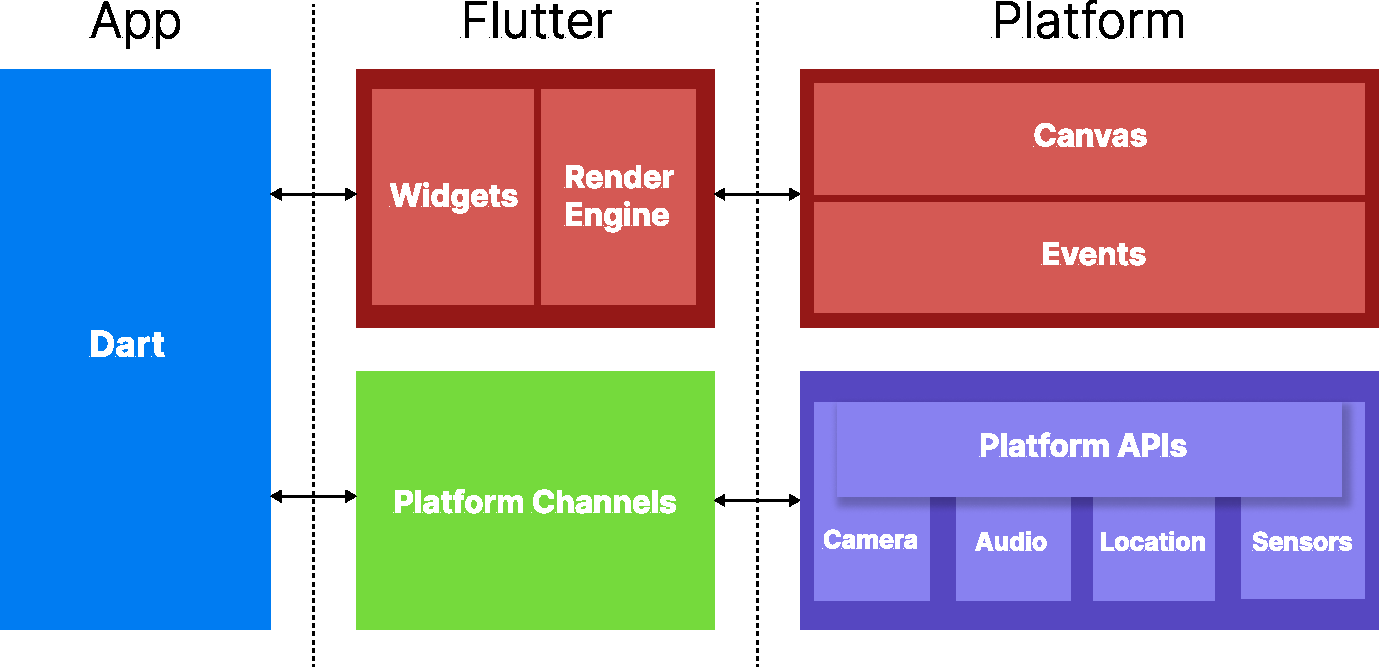
\includegraphics[width=0.9\textwidth]{images/FlutterDiagram@2x.pdf}
    \caption{Authentication Flow: Firebase Authentication integrated with Laravel Sanctum}
\end{figure}

\vspace{0.5cm}

\begin{figure}[H]
    \centering
    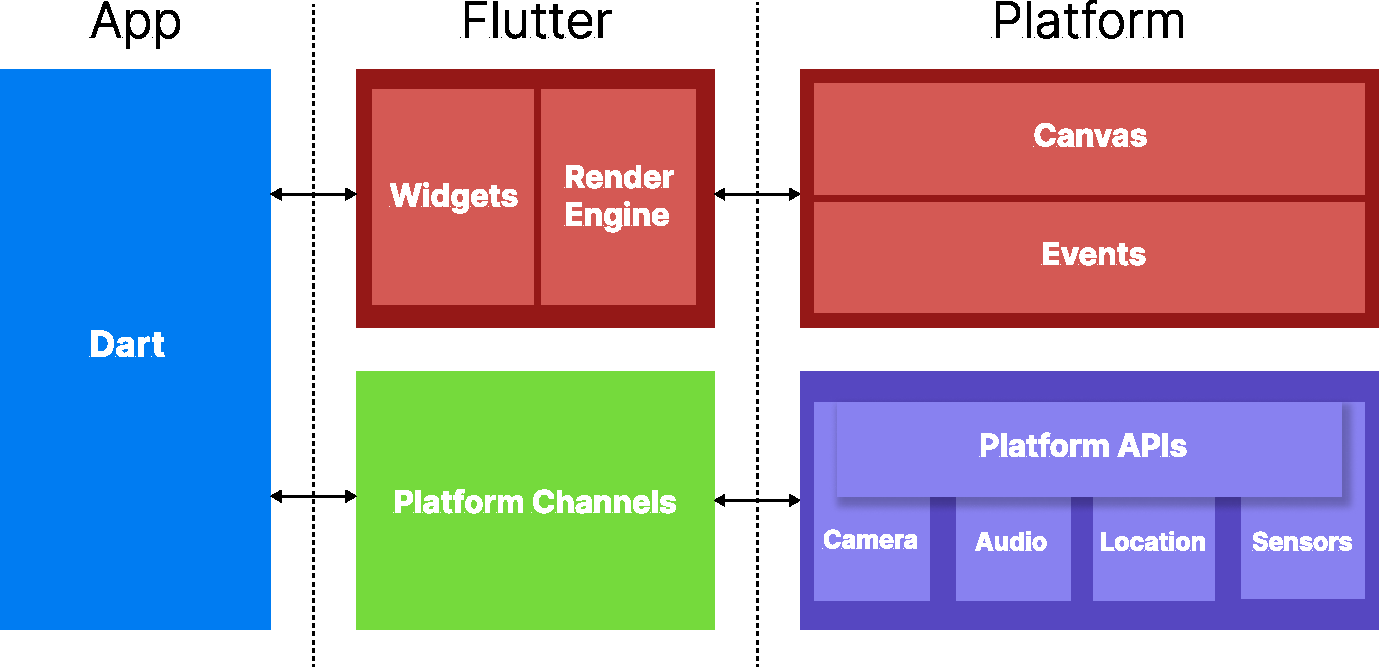
\includegraphics[width=0.9\textwidth]{images/FlutterDiagram@2x.pdf}
    \caption{Role-Based Access Control: Enforcing Permissions for Users, Doctors, Clinics, and Admins}
\end{figure}

\vspace{0.5cm}

With a secure authentication and access control system in place, the structure of our database becomes the backbone for managing and organizing user-related data. To illustrate how different types of users and their interactions are handled within the system, we now highlight the most important tables—such as \texttt{users}, \texttt{clinics}, \texttt{doctors}, and \texttt{appointments}. These tables represent the core entities and relationships that power the application’s functionality.

\vspace{0.5cm}

\begin{figure}[H]
    \centering
    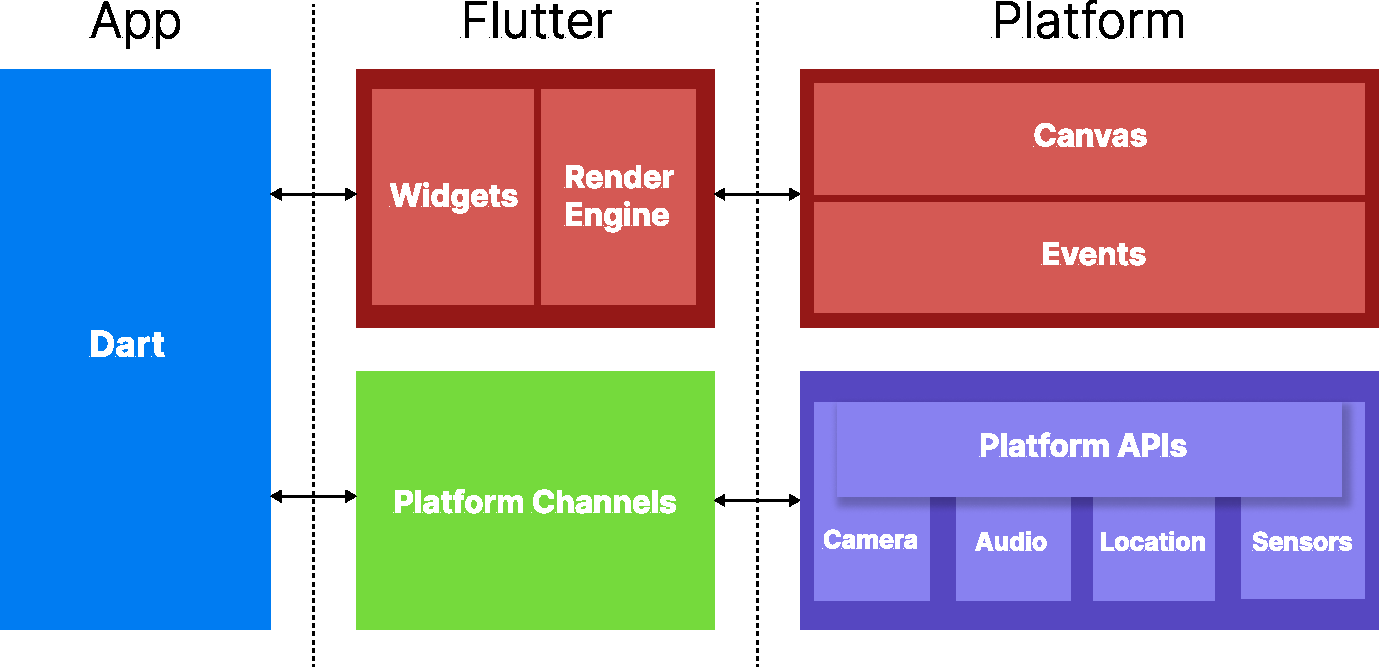
\includegraphics[width=0.9\textwidth]{images/FlutterDiagram@2x.pdf}
    \caption{Users Table Schema}
\end{figure}

\vspace{0.5cm}

\begin{figure}[H]
    \centering
    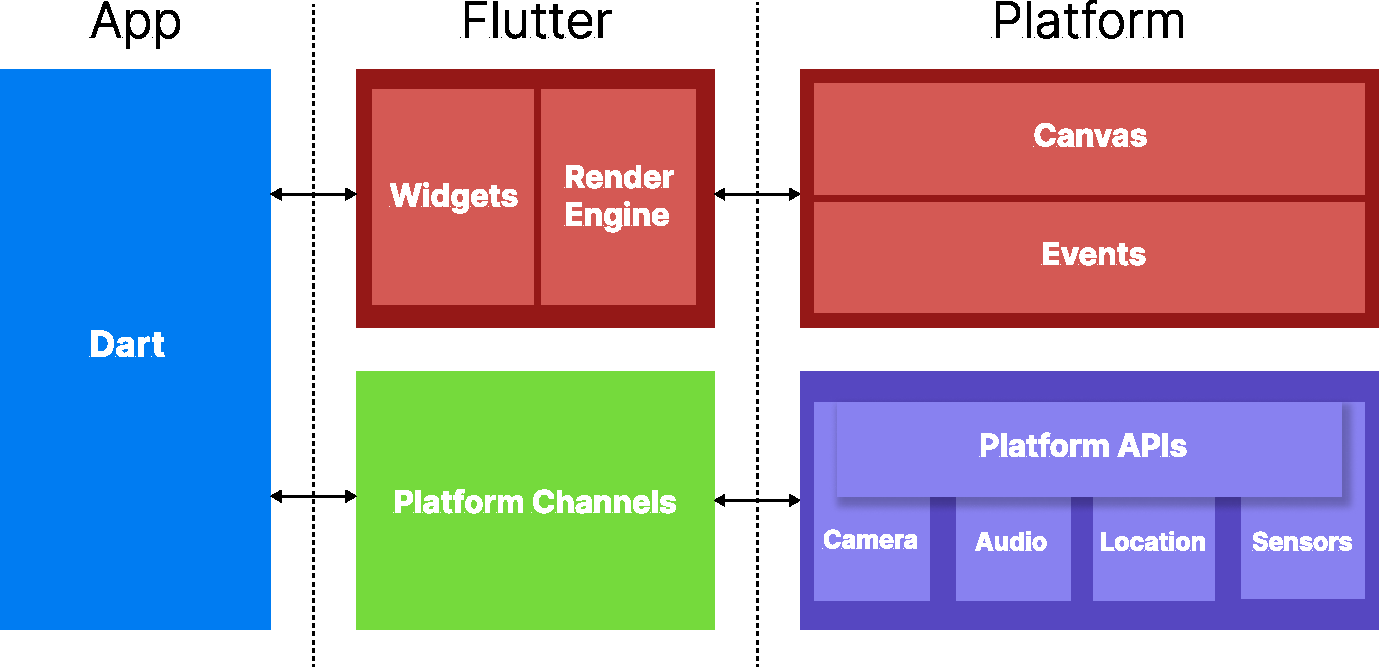
\includegraphics[width=0.9\textwidth]{images/FlutterDiagram@2x.pdf}    \caption{Clinics Table Schema}
\end{figure}

\vspace{0.5cm}

\begin{figure}[H]
    \centering
    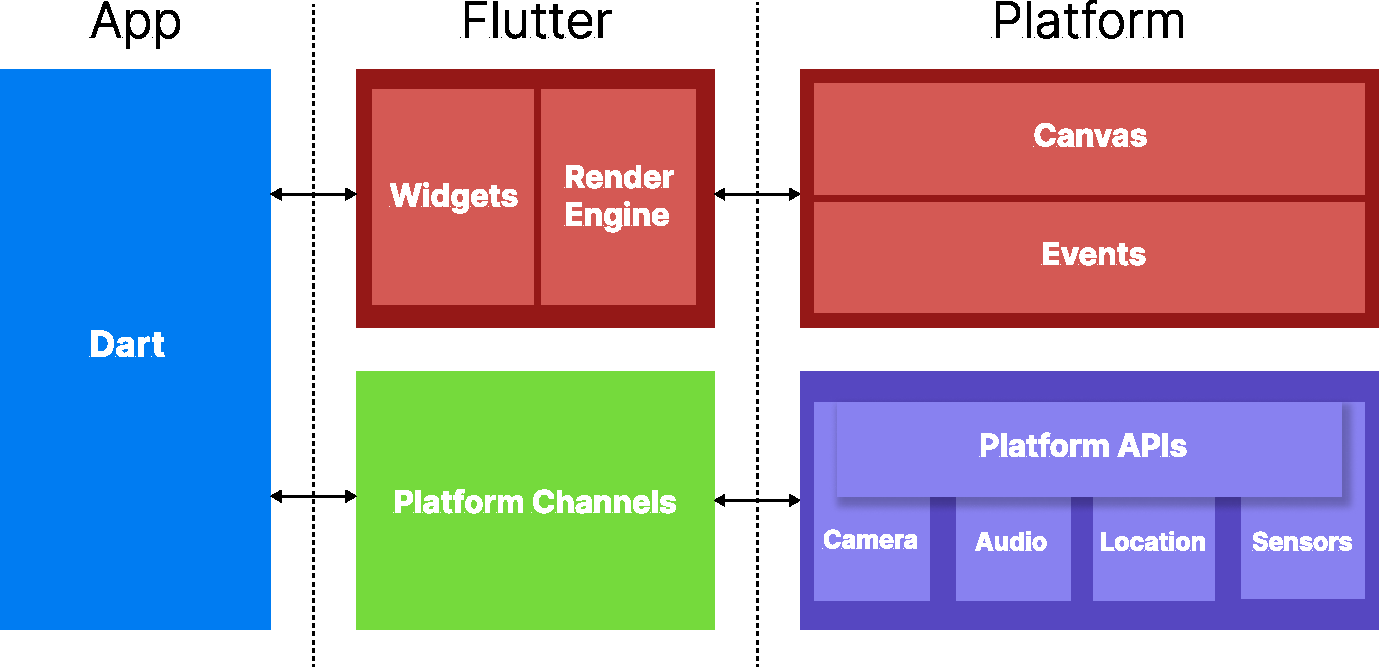
\includegraphics[width=0.9\textwidth]{images/FlutterDiagram@2x.pdf}    \caption{Doctors Table Schema}
\end{figure}

\vspace{0.5cm}

\begin{figure}[H]
    \centering
    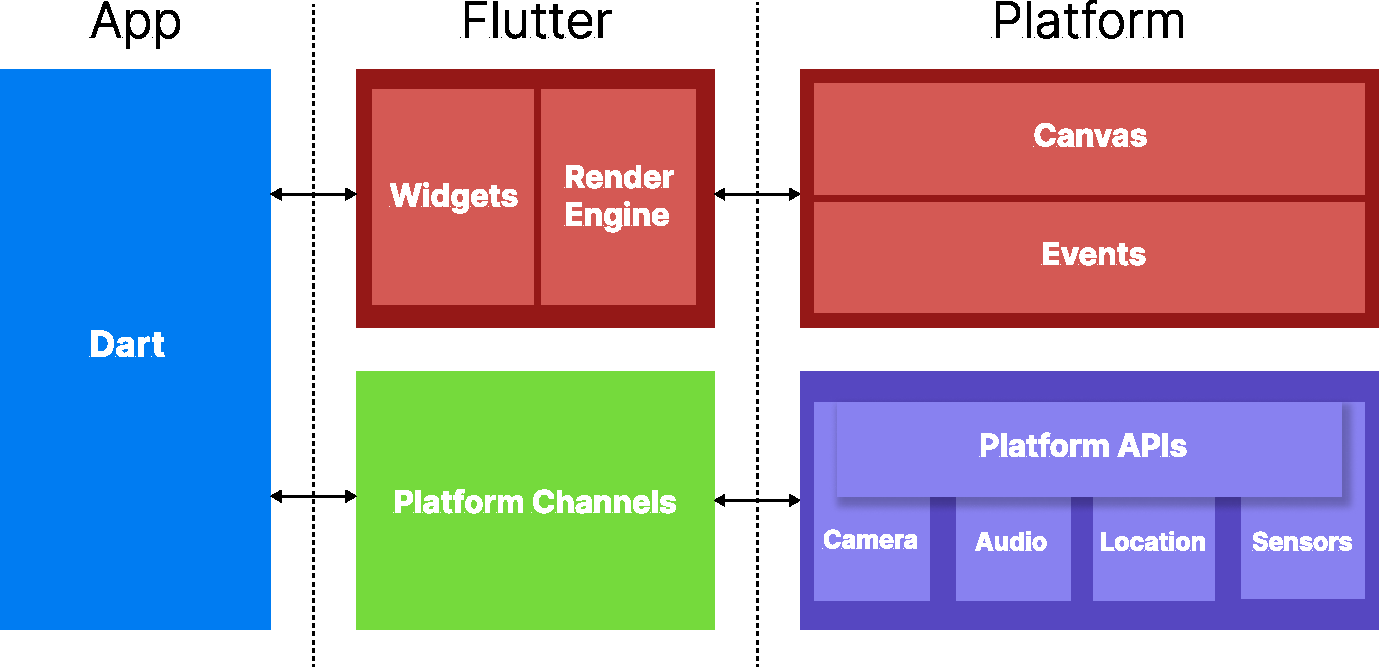
\includegraphics[width=0.9\textwidth]{images/FlutterDiagram@2x.pdf}    \caption{Appointments Table Schema}
\end{figure}

\vspace{0.5cm}

Finally, the complete database structure and its initial data were deployed using the following Artisan command:

\begin{lstlisting}[style=darkbash, language=bash, caption={Laravel command to run migrations and seeders}]
php artisan migrate --seed
\end{lstlisting}

This command runs all migration files to create the defined schema and immediately executes the seeders to populate the tables with required data. It ensures the database is fully prepared for integration with the rest of the application.

\vspace{0.8cm}

\begin{figure}[H]
    \centering
    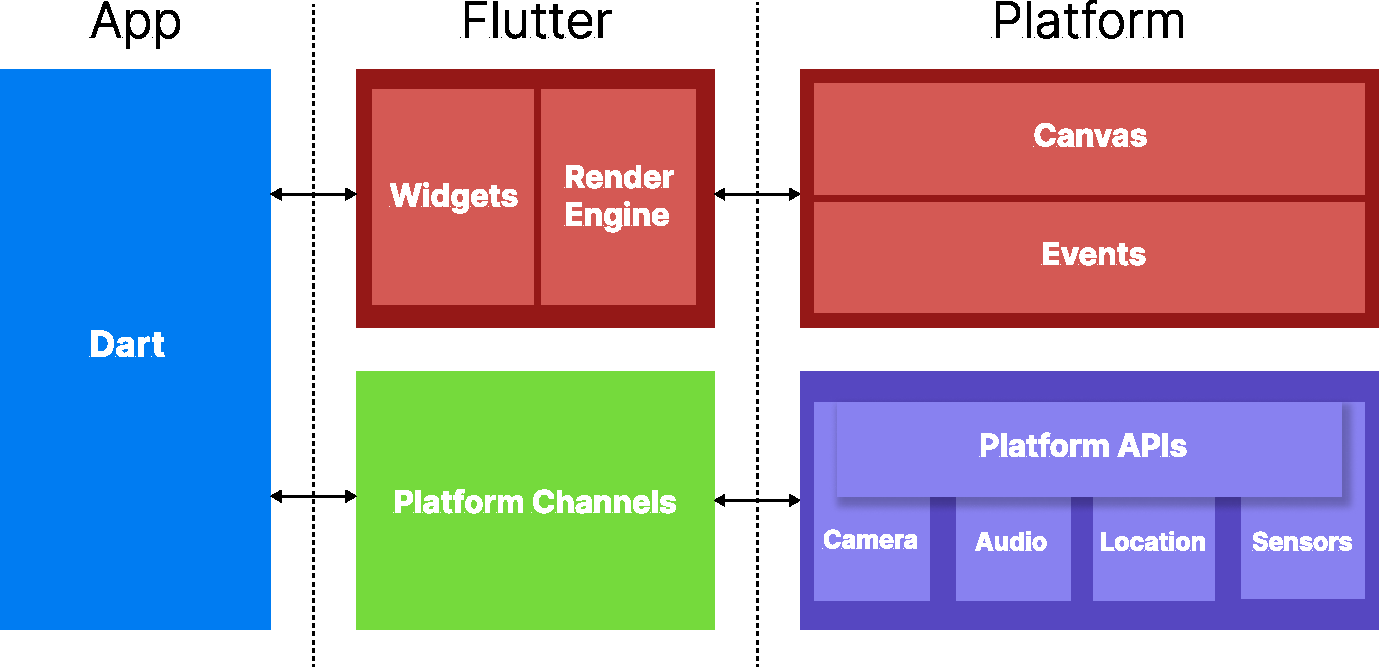
\includegraphics[width=0.85\textwidth]{images/FlutterDiagram@2x.pdf}
    \caption{Laravel MVC Architecture: Model-View-Controller Structure}
\end{figure}


\end{document}


% TODO: MODIFY ADMIN AND REPLACE IT WITH CLINICS in sequence database 



